\documentclass[12pt, oneside]{article}

\usepackage[letterpaper, scale=0.8, centering]{geometry}
\usepackage{fancyhdr}
\setlength{\parindent}{0em}
\setlength{\parskip}{1em}

\pagestyle{fancy}
\fancyhf{}
\renewcommand{\headrulewidth}{0pt}
\rfoot{{\footnotesize Copyright Mia Minnes, 2024, Version \today~(\thepage)}}

\usepackage{titlesec}

\author{CSE105W24}

\newcommand{\instructions}{{\bf For all HW assignments:} Weekly homework 
may be done individually or in groups of up to 3 students. 
You may switch HW partners for different HW assignments. 
Please ensure your name(s) and PID(s) are clearly visible on the first page of your homework submission 
and then upload the PDF to Gradescope. If working in a group, submit only one submission per group: 
one partner uploads the submission through their Gradescope account and then adds the other group member(s) 
to the Gradescope submission by selecting their name(s) in the ``Add Group Members" dialog box. 
You will need to re-add your group member(s) every time you resubmit a new version of your assignment.
 Each homework question will be graded either for correctness (including clear and precise explanations and 
 justifications of all answers) or fair effort completeness. You may only collaborate on ``graded for correctness''
 questions with CSE 105 students in your group; if your group has questions about a problem, you may ask in drop-in 
 help hours or post a private post (visible only to the Instructors) on Piazza.

All submitted homework for this class must be typed. 
You can use a word processing editor if you like (Microsoft Word, Open Office, Notepad, Vim, Google Docs, etc.) 
but you might find it useful to take this opportunity to learn LaTeX. 
LaTeX is a markup language used widely in computer science and mathematics. 
The homework assignments are typed using LaTeX and you can use the source files 
as templates for typesetting your solutions.
To generate state diagrams of machines, we recommend using Flap.js
or JFLAP. Photographs of clearly hand-drawn diagrams may also be used. We recommend that you
submit early drafts to Gradescope so that in case of any technical difficulties, at least some of your
work is present. You may update your submission as many times as you'd like up to the deadline.


{\bf Integrity reminders}
\begin{itemize}
\item Problems should be solved together, not divided up between the partners. The homework is
designed to give you practice with the main concepts and techniques of the course, 
while getting to know and learn from your classmates.
\item You may not collaborate on homework questions graded for correctness with anyone other than your group members.
You may ask questions about the homework in office hours (of the instructor, TAs, and/or tutors) and 
on Piazza (as private notes viewable only to the Instructors).  
You \emph{cannot} use any online resources about the course content other than the class material 
from this quarter -- this is primarily to ensure that we all use consistent notation and
definitions (aligned with the textbook) and also to protect the learning experience you will have when
the `aha' moments of solving the problem authentically happen.
\item Do not share written solutions or partial solutions for homework with 
other students in the class who are not in your group. Doing so would dilute their learning 
experience and detract from their success in the class.
\end{itemize}

}

\newcommand{\gradeCorrect}{({\it Graded for correctness}) }
\newcommand{\gradeCorrectFirst}{\gradeCorrect\footnote{This means your solution 
will be evaluated not only on the correctness of your answers, but on your ability
to present your ideas clearly and logically. You should explain how you 
arrived at your conclusions, using
mathematically sound reasoning. Whether you use formal proof techniques or 
write a more informal argument
for why something is true, your answers should always be well-supported. 
Your goal should be to convince the
reader that your results and methods are sound.} }
\newcommand{\gradeComplete}{({\it Graded for completeness}) }
\newcommand{\gradeCompleteFirst}{\gradeComplete\footnote{This means you will 
get full credit so long as your submission demonstrates honest effort to 
answer the question. You will not be penalized for incorrect answers. 
To demonstrate your honest effort in answering the question, we 
expect you to include your attempt to answer *each* part of the question. 
If you get stuck with your attempt, you can still demonstrate 
your effort by explaining where you got stuck and what 
you did to try to get unstuck.} }

\usepackage{tikz}
\usetikzlibrary{automata,positioning,arrows}

\usepackage{amssymb,amsmath,pifont,amsfonts,comment,enumerate,enumitem}
\usepackage{currfile,xstring,hyperref,tabularx,graphicx,wasysym}
\usepackage[labelformat=empty]{caption}
\usepackage{xcolor}
\usepackage{multicol,multirow,array,listings,tabularx,lastpage,textcomp,booktabs}

\lstnewenvironment{algorithm}[1][] {   
    \lstset{ mathescape=true,
        frame=tB,
        numbers=left, 
        numberstyle=\tiny,
        basicstyle=\rmfamily\scriptsize, 
        keywordstyle=\color{black}\bfseries,
        keywords={,procedure, div, for, to, input, output, return, datatype, function, in, if, else, foreach, while, begin, end, }
        numbers=left,
        xleftmargin=.04\textwidth,
        #1
    }
}
{}

\newcommand\abs[1]{\lvert~#1~\rvert}
\newcommand{\st}{\mid}

\newcommand{\cmark}{\ding{51}}
\newcommand{\xmark}{\ding{55}}
 
\newcommand{\SUBSTRING}{\textsc{Substring}}
\newcommand{\REP}{\textsc{Rep}}
\newcommand{\blank}{\scalebox{1.5}{\textvisiblespace}}
 
\title{HW1CSE105W24: Homework assignment 1}
\date{Due: January 18th at 5pm (no penalty late submission until 8am next morning), via Gradescope}


\begin{document}
\maketitle
\thispagestyle{fancy}

{\bf In this assignment,}

You will practice reading and
applying the definitions of alphabets, strings, languages, Kleene star, and regular expressions.
You will use regular expressions and relate them to languages and finite automata.
You will use precise notation to formally define the state diagram of finite automata,
and you will use clear English to describe computations of finite automata informally.


{\bf Resources}: To review the topics 
for this assignment, see the class material from Week 1.
We will post frequently asked questions and our answers to them in a 
pinned Piazza post.

{\bf Reading and extra practice problems}: Sipser Section 0, 1.3, 1.1.
Chapter 1 exercises 1.1, 1.2, 1.3, 1.18, 1.23.

\instructions

You will submit this assignment via Gradescope
(\href{https://www.gradescope.com}{https://www.gradescope.com}) 
in the assignment called ``hw1CSE105W24''.

{\bf Assigned questions}
\begin{enumerate}[wide, labelwidth=!, labelindent=0pt]
\item\gradeCompleteFirst \textbf{Finding examples and edge cases} (12 points):

With $\Sigma_1 = \{0,1\}$ and 
$\Sigma_2 = \{a,b,c,d,e,f,g,h,i,j,k,l,m,n,o,p,q,r,s,t,u,v,w,x,y,z\}$
and $\Gamma = \{0,1,x,y,z\}$

    \begin{enumerate}
    \item Give an example of the shortest string over $\Sigma_1$ that is meaningful to you in some way, and explain 
    why it's meaningful to you.

    \item List all examples of strings of length $1$ over $\Sigma_2$ and explain why your list is exhaustive.

    \item Calculate the number of distinct strings of length 3 over $\Gamma$ and explain your calculation.

    \item With the ordering $x < y < z < 0 < 1$, list the first ten strings over $\Gamma$ in string order.

    \item Give an example of a finite set that is a language over $\Sigma_1$ and over $\Sigma_2$ and over $\Gamma$, 
    or explain why there is no such set.
    
    \item  Give an example of an infinite set that is a language over $\Sigma_1$  and over $\Gamma$, 
    or explain why there is no such set.

    \end{enumerate}

\item\gradeComplete \textbf{Regular expressions} (10 points):

    \begin{enumerate}
    \item Give three regular expressions that all describe the set of all strings over $\{a,b\}$ that have 
    even length. Ungraded bonus challenge: Make the expressions as different as possible!

    \item A friend tells you that each regular expression that has a Kleene star ($~^*$) describes an
    infinite language. Are they right? Either help them justify their claim or give a counterexample to disprove it
    and then fix the formula.

    \end{enumerate}

\item\gradeCorrectFirst \textbf{Functions over languages} (15 points):

For languages $L_1, L_2$ over the alphabet $\Sigma_1 = \{0,1\}$, we have the 
associated sets of strings
\[
    SUBSTRING(L_1) = \{ w \in \Sigma_1^* ~|~ \text{there exist } a,b \in \Sigma_1^* \text{ such that } awb \in L_1\}
\]
and 
\[
    L_1 \circ L_2 = \{ w \in \Sigma_1^* ~|~ w = uv \text{ for some strings } u \in L_1 \text{ and } v \in L_2 \}
\]
    \begin{enumerate}
    \item Specify an example language $A$ over $\Sigma_1$ such that 
    $A \neq \emptyset$ and yet $\SUBSTRING(A) = \emptyset$, 
    or explain why there is no such example. 
    A complete solution will include either (1) a precise and
    clear description of your example language $A$ 
    and a precise and clear description of
    the result of computing $\SUBSTRING(A)$ using relevant definitions 
    to justify this description and to justify the set equality with 
    $\emptyset$, or (2) a sufficiently general and correct argument
    why there is no such example, referring back to the relevant definitions.

    \item Specify example languages $B, C$ over $\Sigma_1$ such that 
    $B \neq \Sigma_1^*$ and $C \neq \Sigma_1^*$ and yet $B \circ C = \Sigma_1^*$, 
    or explain why there are no such examples. 
    A complete solution will include either (1) a precise and
    clear description of your example languages $B,C$ 
    and a precise and clear description of
    the result of computing $B \circ C$ using relevant definitions 
    to justify this description and to justify the set equality with 
    $\Sigma_1^*$, or (2) a sufficiently general and correct argument
    why there is no such example, referring back to the relevant definitions.

    \item Specify example {\bf finite} languages $L_1, L_2$ over $\Sigma_1$ such that 
    $L_1 \circ L_2 \neq L_1$ but $|L_1 \circ L_2| = |L_1|$, or 
    explain why there are no such examples.
    A complete solution will include either (1) a precise and
    clear description of your example languages $L_1, L_2$ 
    and a precise and clear description of
    the result of computing $L_1 \circ L_2$ using relevant definitions 
    to justify this description and to justify the cardinality claims and set (in)equality claims, 
    or (2) a sufficiently general and correct argument
    why there is no such example, referring back to the relevant definitions.
    \end{enumerate}


\item\gradeCorrect \textbf{Finite automata} (13 points):

Consider the finite automaton $(Q, \Sigma, \delta, q_0, F)$ whose state diagram is depicted below
\begin{center}
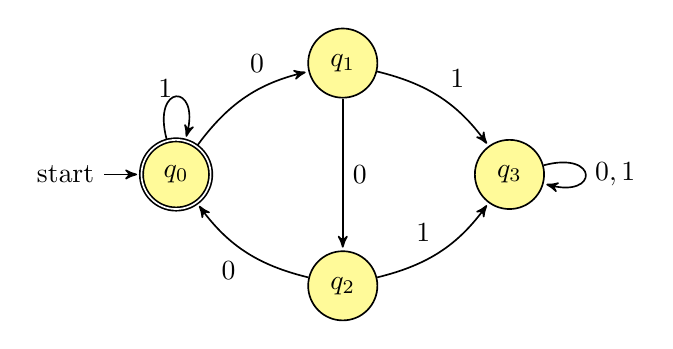
\begin{tikzpicture}[->,>=stealth',shorten >=1pt, auto, node distance=2cm, semithick]
\tikzstyle{every state}=[text=black, fill=yellow!40]

\node[initial,state, accepting] (q0)          {$q_0$};
\node[state]         (q1) [above right of=q0, xshift=20pt] {$q_1$};
\node[state]         (q2) [below right of=q0, xshift=20pt] {$q_2$};
\node[state]         (q3) [below right of=q1, xshift=20pt] {$q_3$};

\path (q0) edge  [loop above, near start] node {$1$} (q0)
        edge [bend left=20, near end] node {$0$} (q1)
    (q1) edge [bend left=0] node {$0$} (q2)
        edge [bend left=20] node {$1$} (q3)
    (q2) edge [bend left=20] node {$0$} (q0)
        edge [bend right=20] node {$1$} (q3)
    (q3) edge [loop right] node {$0,1$} (q3)
;
\end{tikzpicture}
\end{center}
where $Q = \{q_0, q_1, q_2, q_3\}$, $\Sigma = \{0,1\}$, and $F = \{q_0\}$, and $\delta: Q \times \Sigma \to Q$
is specified by the look-up table
\begin{center}
\begin{tabular}{c|cc}
        & $0$ & $1$ \\
    \hline
  $q_0$ & $q_1$ & $q_0$ \\
  $q_1$ & $q_2$ & $q_3$ \\
  $q_2$ & $q_0$ & $q_3$ \\
  $q_3$ & $q_3$ & $q_3$
\end{tabular}
\end{center}
    \begin{enumerate}
    \item  A friend tries to summarize the transition function with the formula
    \[
        \delta(q_i,x) = \begin{cases}
            q_0 &\text{ when $i=0$ and $x=1$} \\
            q_3 &\text{ when $0<i\leq 3$ and $x=1$}\\
            q_j &\text{ when $j = (i+1) \mod 3$ and $x=0$}
        \end{cases}
    \]
    Are they right? Either help them justify their claim or give a counterexample to disprove it and then 
    fix their formula.

    \item Give a regular expression $R$ so that $L(R)$ is the language 
    recognized by this finite automaton. Justify your answer by referring to the 
    definition of the semantics of regular expressions and computations of finite automata. 
    Include an explanation for why each string in $L(R)$ is accepted by the finite automaton {\it and}
    for why each string not in $L(R)$ is rejected by the finite automaton.

    \item  Keeping the same set of states $Q = \{q_0, q_1, q_2, q_3\}$, alphabet $\Sigma = \{0,1\}$, 
    same start state $q_0$, and same transition 
    function $\delta$, choose a new set of accepting states $F_{new}$ so that the new 
    finite automaton that results accepts at least one string that the original one rejected {\bf and} rejects
    at least one string that the original one accepted, or explain why there is no such choice of $F_{new}$.
    A complete solution will include either (1) a precise and
    clear description of your choice of $F_{new}$
    and a precise and clear the two example strings using relevant definitions 
    to justify them, or (2) a sufficiently general and correct argument
    why there is no such example, referring back to the relevant definitions.

    \end{enumerate}
    
    \end{enumerate}
\newpage
\titleformat{\subsubsection}[runin]
   {\normalfont\bfseries}{}{}{}
   
\title{ProjectCSE105W24: Project}
\date{Due TBD at 5pm (no penalty late submission until 8am next day)}


\maketitle

\thispagestyle{fancy}

The project component is designed for you to go deeper and extend your work on assignments 
and to explore an application of your choosing. 
The project is an individual assignment and has TBD tasks: 

\newpage

\end{document}